% Options for packages loaded elsewhere
% Options for packages loaded elsewhere
\PassOptionsToPackage{unicode}{hyperref}
\PassOptionsToPackage{hyphens}{url}
%
\documentclass[
  ignorenonframetext,
]{beamer}
\newif\ifbibliography
\usepackage{pgfpages}
\setbeamertemplate{caption}[numbered]
\setbeamertemplate{caption label separator}{: }
\setbeamercolor{caption name}{fg=normal text.fg}
\beamertemplatenavigationsymbolsempty
% remove section numbering
\setbeamertemplate{part page}{
  \centering
  \begin{beamercolorbox}[sep=16pt,center]{part title}
    \usebeamerfont{part title}\insertpart\par
  \end{beamercolorbox}
}
\setbeamertemplate{section page}{
  \centering
  \begin{beamercolorbox}[sep=12pt,center]{section title}
    \usebeamerfont{section title}\insertsection\par
  \end{beamercolorbox}
}
\setbeamertemplate{subsection page}{
  \centering
  \begin{beamercolorbox}[sep=8pt,center]{subsection title}
    \usebeamerfont{subsection title}\insertsubsection\par
  \end{beamercolorbox}
}
% Prevent slide breaks in the middle of a paragraph
\widowpenalties 1 10000
\raggedbottom
\AtBeginPart{
  \frame{\partpage}
}
\AtBeginSection{
  \ifbibliography
  \else
    \frame{\sectionpage}
  \fi
}
\AtBeginSubsection{
  \frame{\subsectionpage}
}
\usepackage{iftex}
\ifPDFTeX
  \usepackage[T1]{fontenc}
  \usepackage[utf8]{inputenc}
  \usepackage{textcomp} % provide euro and other symbols
\else % if luatex or xetex
  \usepackage{unicode-math} % this also loads fontspec
  \defaultfontfeatures{Scale=MatchLowercase}
  \defaultfontfeatures[\rmfamily]{Ligatures=TeX,Scale=1}
\fi
\usepackage{lmodern}

\ifPDFTeX\else
  % xetex/luatex font selection
\fi
% Use upquote if available, for straight quotes in verbatim environments
\IfFileExists{upquote.sty}{\usepackage{upquote}}{}
\IfFileExists{microtype.sty}{% use microtype if available
  \usepackage[]{microtype}
  \UseMicrotypeSet[protrusion]{basicmath} % disable protrusion for tt fonts
}{}
\makeatletter
\@ifundefined{KOMAClassName}{% if non-KOMA class
  \IfFileExists{parskip.sty}{%
    \usepackage{parskip}
  }{% else
    \setlength{\parindent}{0pt}
    \setlength{\parskip}{6pt plus 2pt minus 1pt}}
}{% if KOMA class
  \KOMAoptions{parskip=half}}
\makeatother

\usepackage{color}
\usepackage{fancyvrb}
\newcommand{\VerbBar}{|}
\newcommand{\VERB}{\Verb[commandchars=\\\{\}]}
\DefineVerbatimEnvironment{Highlighting}{Verbatim}{commandchars=\\\{\}}
% Add ',fontsize=\small' for more characters per line
\usepackage{framed}
\definecolor{shadecolor}{RGB}{241,243,245}
\newenvironment{Shaded}{\begin{snugshade}}{\end{snugshade}}
\newcommand{\AlertTok}[1]{\textcolor[rgb]{0.68,0.00,0.00}{#1}}
\newcommand{\AnnotationTok}[1]{\textcolor[rgb]{0.37,0.37,0.37}{#1}}
\newcommand{\AttributeTok}[1]{\textcolor[rgb]{0.40,0.45,0.13}{#1}}
\newcommand{\BaseNTok}[1]{\textcolor[rgb]{0.68,0.00,0.00}{#1}}
\newcommand{\BuiltInTok}[1]{\textcolor[rgb]{0.00,0.23,0.31}{#1}}
\newcommand{\CharTok}[1]{\textcolor[rgb]{0.13,0.47,0.30}{#1}}
\newcommand{\CommentTok}[1]{\textcolor[rgb]{0.37,0.37,0.37}{#1}}
\newcommand{\CommentVarTok}[1]{\textcolor[rgb]{0.37,0.37,0.37}{\textit{#1}}}
\newcommand{\ConstantTok}[1]{\textcolor[rgb]{0.56,0.35,0.01}{#1}}
\newcommand{\ControlFlowTok}[1]{\textcolor[rgb]{0.00,0.23,0.31}{\textbf{#1}}}
\newcommand{\DataTypeTok}[1]{\textcolor[rgb]{0.68,0.00,0.00}{#1}}
\newcommand{\DecValTok}[1]{\textcolor[rgb]{0.68,0.00,0.00}{#1}}
\newcommand{\DocumentationTok}[1]{\textcolor[rgb]{0.37,0.37,0.37}{\textit{#1}}}
\newcommand{\ErrorTok}[1]{\textcolor[rgb]{0.68,0.00,0.00}{#1}}
\newcommand{\ExtensionTok}[1]{\textcolor[rgb]{0.00,0.23,0.31}{#1}}
\newcommand{\FloatTok}[1]{\textcolor[rgb]{0.68,0.00,0.00}{#1}}
\newcommand{\FunctionTok}[1]{\textcolor[rgb]{0.28,0.35,0.67}{#1}}
\newcommand{\ImportTok}[1]{\textcolor[rgb]{0.00,0.46,0.62}{#1}}
\newcommand{\InformationTok}[1]{\textcolor[rgb]{0.37,0.37,0.37}{#1}}
\newcommand{\KeywordTok}[1]{\textcolor[rgb]{0.00,0.23,0.31}{\textbf{#1}}}
\newcommand{\NormalTok}[1]{\textcolor[rgb]{0.00,0.23,0.31}{#1}}
\newcommand{\OperatorTok}[1]{\textcolor[rgb]{0.37,0.37,0.37}{#1}}
\newcommand{\OtherTok}[1]{\textcolor[rgb]{0.00,0.23,0.31}{#1}}
\newcommand{\PreprocessorTok}[1]{\textcolor[rgb]{0.68,0.00,0.00}{#1}}
\newcommand{\RegionMarkerTok}[1]{\textcolor[rgb]{0.00,0.23,0.31}{#1}}
\newcommand{\SpecialCharTok}[1]{\textcolor[rgb]{0.37,0.37,0.37}{#1}}
\newcommand{\SpecialStringTok}[1]{\textcolor[rgb]{0.13,0.47,0.30}{#1}}
\newcommand{\StringTok}[1]{\textcolor[rgb]{0.13,0.47,0.30}{#1}}
\newcommand{\VariableTok}[1]{\textcolor[rgb]{0.07,0.07,0.07}{#1}}
\newcommand{\VerbatimStringTok}[1]{\textcolor[rgb]{0.13,0.47,0.30}{#1}}
\newcommand{\WarningTok}[1]{\textcolor[rgb]{0.37,0.37,0.37}{\textit{#1}}}

\usepackage{longtable,booktabs,array}
\usepackage{calc} % for calculating minipage widths
\usepackage{caption}
% Make caption package work with longtable
\makeatletter
\def\fnum@table{\tablename~\thetable}
\makeatother
\usepackage{graphicx}
\makeatletter
\newsavebox\pandoc@box
\newcommand*\pandocbounded[1]{% scales image to fit in text height/width
  \sbox\pandoc@box{#1}%
  \Gscale@div\@tempa{\textheight}{\dimexpr\ht\pandoc@box+\dp\pandoc@box\relax}%
  \Gscale@div\@tempb{\linewidth}{\wd\pandoc@box}%
  \ifdim\@tempb\p@<\@tempa\p@\let\@tempa\@tempb\fi% select the smaller of both
  \ifdim\@tempa\p@<\p@\scalebox{\@tempa}{\usebox\pandoc@box}%
  \else\usebox{\pandoc@box}%
  \fi%
}
% Set default figure placement to htbp
\def\fps@figure{htbp}
\makeatother

\ifLuaTeX
  \usepackage{luacolor}
  \usepackage[soul]{lua-ul}
\else
  \usepackage{soul}
  \makeatletter
  \let\HL\hl
  \renewcommand\hl{% fix for beamer highlighting
    \let\set@color\beamerorig@set@color
    \let\reset@color\beamerorig@reset@color
    \HL}
  \makeatother
\fi




\setlength{\emergencystretch}{3em} % prevent overfull lines

\providecommand{\tightlist}{%
  \setlength{\itemsep}{0pt}\setlength{\parskip}{0pt}}



 


\makeatletter
\@ifpackageloaded{caption}{}{\usepackage{caption}}
\AtBeginDocument{%
\ifdefined\contentsname
  \renewcommand*\contentsname{Table of contents}
\else
  \newcommand\contentsname{Table of contents}
\fi
\ifdefined\listfigurename
  \renewcommand*\listfigurename{List of Figures}
\else
  \newcommand\listfigurename{List of Figures}
\fi
\ifdefined\listtablename
  \renewcommand*\listtablename{List of Tables}
\else
  \newcommand\listtablename{List of Tables}
\fi
\ifdefined\figurename
  \renewcommand*\figurename{Figure}
\else
  \newcommand\figurename{Figure}
\fi
\ifdefined\tablename
  \renewcommand*\tablename{Table}
\else
  \newcommand\tablename{Table}
\fi
}
\@ifpackageloaded{float}{}{\usepackage{float}}
\floatstyle{ruled}
\@ifundefined{c@chapter}{\newfloat{codelisting}{h}{lop}}{\newfloat{codelisting}{h}{lop}[chapter]}
\floatname{codelisting}{Listing}
\newcommand*\listoflistings{\listof{codelisting}{List of Listings}}
\makeatother
\makeatletter
\makeatother
\makeatletter
\@ifpackageloaded{caption}{}{\usepackage{caption}}
\@ifpackageloaded{subcaption}{}{\usepackage{subcaption}}
\makeatother

\usepackage{bookmark}
\IfFileExists{xurl.sty}{\usepackage{xurl}}{} % add URL line breaks if available
\urlstyle{same}
\hypersetup{
  pdftitle={Buscando EL lugar de la mancha},
  pdfauthor={Victoria Ruiz Parrado},
  hidelinks,
  pdfcreator={LaTeX via pandoc}}


\title{Buscando EL lugar de la mancha}
\author{Victoria Ruiz Parrado}
\date{}

\begin{document}
\frame{\titlepage}

\renewcommand*\contentsname{Table of contents}
\begin{frame}[allowframebreaks]
  \frametitle{Table of contents}
  \setcounter{tocdepth}{3}
  \tableofcontents
\end{frame}
\setcounter{tocdepth}{3}
\tableofcontents
}

\begin{frame}{¿Es Villanueva de los Infantes El lugar de La Mancha?}
\phantomsection\label{sec-intro}
\begin{figure}

\centering{

\pandocbounded{\includegraphics[keepaspectratio]{presentacion_quijote_ppt_files/mediabag/Quijote2.png}}

}

\caption{\label{fig-quijote}}

\end{figure}%
\end{frame}

\begin{frame}{Texto El Quijote}
\phantomsection\label{texto-el-quijote}
\ul{\emph{En un lugar de la
Mancha}}\textsuperscript{\href{https://cvc.cervantes.es/literatura/clasicos/quijote/edicion/parte1/cap01/default.htm\#np2n}{\textbf{\emph{2}}}}\emph{,
de cuyo nombre no quiero
acordarme\textsuperscript{\href{https://cvc.cervantes.es/literatura/clasicos/quijote/edicion/parte1/cap01/default.htm\#np3n}{3}},
no ha mucho tiempo que vivía un hidalgo de los de lanza en astillero,
adarga antigua, rocín flaco y galgo
corredor\textsuperscript{\href{https://cvc.cervantes.es/literatura/clasicos/quijote/edicion/parte1/cap01/default.htm\#np4n}{4}}.
Una olla de algo más vaca que carnero, salpicón las más
noches\textsuperscript{\href{https://cvc.cervantes.es/literatura/clasicos/quijote/edicion/parte1/cap01/default.htm\#np5n}{5}},
duelos y quebrantos los
sábados\textsuperscript{\href{https://cvc.cervantes.es/literatura/clasicos/quijote/edicion/parte1/cap01/default.htm\#np6n}{6}},
lantejas los
viernes\textsuperscript{\href{https://cvc.cervantes.es/literatura/clasicos/quijote/edicion/parte1/cap01/default.htm\#np7n}{7}},
algún palomino de añadidura los
domingos\textsuperscript{\href{https://cvc.cervantes.es/literatura/clasicos/quijote/edicion/parte1/cap01/default.htm\#np8n}{8}},
consumían las tres partes de su
hacienda\textsuperscript{\href{https://cvc.cervantes.es/literatura/clasicos/quijote/edicion/parte1/cap01/default.htm\#np9n}{9}}.
El resto della concluían sayo de
velarte\textsuperscript{\href{https://cvc.cervantes.es/literatura/clasicos/quijote/edicion/parte1/cap01/default.htm\#np10n}{10}},
calzas de velludo para las fiestas, con sus pantuflos de lo
mesmo\textsuperscript{\href{https://cvc.cervantes.es/literatura/clasicos/quijote/edicion/parte1/cap01/default.htm\#np11n}{11}},
y los días de entresemana se honraba con su vellorí de lo más
fino\textsuperscript{\href{https://cvc.cervantes.es/literatura/clasicos/quijote/edicion/parte1/cap01/default.htm\#np12n}{12}}.
Tenía en su casa una ama que pasaba de los cuarenta y una sobrina que no
llegaba a los veinte, y un mozo de campo y plaza que así ensillaba el
rocín como tomaba la
podadera\textsuperscript{\href{https://cvc.cervantes.es/literatura/clasicos/quijote/edicion/parte1/cap01/default.htm\#np13n}{13}}.
Frisaba la edad de nuestro hidalgo con los cincuenta
años\textsuperscript{\href{https://cvc.cervantes.es/literatura/clasicos/quijote/edicion/parte1/cap01/default.htm\#np14n}{14}}.
Era de complexión recia, seco de carnes, enjuto de
rostro\textsuperscript{\href{https://cvc.cervantes.es/literatura/clasicos/quijote/edicion/parte1/cap01/default.htm\#np15n}{15}},
gran madrugador y amigo de la caza. Quieren decir que tenía el
sobrenombre de «Quijada», o «Quesada», que en esto hay alguna diferencia
en los autores que deste caso escriben, aunque por conjeturas
verisímiles\textsuperscript{\href{https://cvc.cervantes.es/literatura/clasicos/quijote/edicion/parte1/cap01/default.htm\#acn2}{II}}
se deja entender que se llamaba
«\textbf{Quijana}»\textsuperscript{\href{https://cvc.cervantes.es/literatura/clasicos/quijote/edicion/parte1/cap01/default.htm\#acn3}{III},~\href{https://cvc.cervantes.es/literatura/clasicos/quijote/edicion/parte1/cap01/default.htm\#np16n}{16}}.
Pero esto importa poco a nuestro cuento: basta que en la narración dél
no se salga un punto de la verdad. (\textbf{libroquijote?})}
\end{frame}

\begin{frame}
Un grupo de investigadores ha recolectado evaluaciones subjetivas de
expertos en literatura, historia y cultura manchega sobre cuatro pueblos
candidatos a ser el famoso ``lugar de La Mancha de cuyo nombre no quiero
acordarme''.

Los \textbf{criterios de evaluación} son:

\{nonincremental\} - Idealismo cervantino

\begin{itemize}
\item
  Ambiente rural que encaja con la novela
\item
  Presencia de tradiciones caballerescas
\item
  Probabilidad histórica percibida
\end{itemize}
\end{frame}

\begin{frame}
Los \textbf{pueblos candidatos} son:

\{.incremental\} - Argamasilla de Alba

\begin{itemize}
\item
  Villanueva de los Infantes
\item
  Campo de Criptana
\item
  El Toboso
\end{itemize}
\end{frame}

\begin{frame}{Mapa de Castilla La Mancha}
\phantomsection\label{sec-mapa}
Para averiguar cual es el verdadero lugar de la mancha, hay que tener en
cuenta el mapa de carreteras de la épica.

La Figure~\ref{fig-mapa} muestra el mapa de Castilla La Mancha que tenía
Don Quijote.

\begin{figure}

\centering{

\pandocbounded{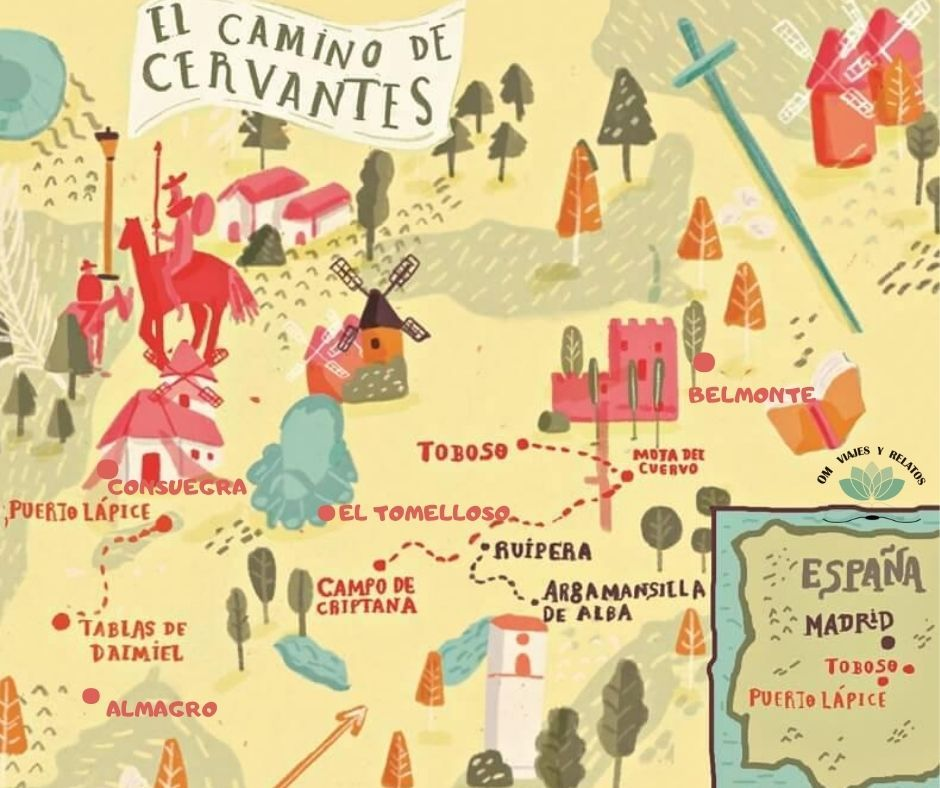
\includegraphics[keepaspectratio]{MAPA-RUTA-QUIJOTE.jpg}}

}

\caption{\label{fig-mapa}Mapa Cervantes}

\end{figure}%

Imagen obtenida de \url{https://omviajesyrelatos.com/}
\end{frame}

\begin{frame}{Descripción distancias}
\phantomsection\label{sec-distancias}
Las distancias se calculan según la fórmula de Euler:

\begin{equation}\phantomsection\label{eq-distancia}{\sqrt{(x_1-x_2)^2+(y_1-y_2)^2}}\end{equation}
\end{frame}

\begin{frame}
Las variables x e y son las coordenadas, y las variables PL, SM, ET y MU
son las distancias de cada pueblo a Puerto Lápice, Sierra Morena y El
Toboso, más la correspondiente al denominado \emph{punto Tarfe
(\textbf{gonzalez2008donde?})}.

\#Datos
\end{frame}

\begin{frame}{Investigación}
\phantomsection\label{sec-investigacion}
Para determinar si Villanueva de los Infantes es el pueblo de Don
Quijote, los investigadores se han hecho las siguientes preguntas:

\begin{itemize}
\item
  ¿Es Argamasilla de Alba percibida como significativamente menos
  idealista que Villanueva de los Infantes?
\item
  ¿Aumenta significativamente la valoración de Villanueva tras leer El
  Quijote?
\item
  ¿Hay diferencias significativas en la percepción ``quijotesca'' entre
  los cuatro pueblos? Si hay diferencias, ¿cuáles destacan?
\item
  ¿Cuál es el criterio más valorado en Villanuev de los Infantes? ¿Las
  diferencias entre criterios son significativas?
\end{itemize}
\end{frame}

\begin{frame}{Pruebas}
\phantomsection\label{sec-pruebas}
Esta sección recoge los datos recopilados para responder a las preguntas
anteriores.

\begin{block}{Prueba 1: Comparación entre la idealidad de dos pueblos}
\phantomsection\label{sec-pruebas1}
\begin{longtable}[]{@{}lll@{}}
\caption{Datos Prueba 1}\label{tbl-prueba1}\tabularnewline
\toprule\noalign{}
Evaluador & Argmasilla & Villanueva de los Infantes \\
\midrule\noalign{}
\endfirsthead
\toprule\noalign{}
Evaluador & Argmasilla & Villanueva de los Infantes \\
\midrule\noalign{}
\endhead
E1 & 8 & 6 \\
E2 & 9 & 5 \\
E3 & 7 & 6 \\
E4 & 8 & 4 \\
E5 & 9 & 5 \\
\bottomrule\noalign{}
\end{longtable}
\end{block}
\end{frame}

\begin{frame}
\begin{block}{Prueba 2: Comparación de la percepción histórica antes y
después de leer el Quijote}
\phantomsection\label{sec-prueba2}
\begin{longtable}[]{@{}lll@{}}
\caption{Datos Prueba 2}\label{tbl-prueba2}\tabularnewline
\toprule\noalign{}
Evaluador & Antes leer & Después Leer \\
\midrule\noalign{}
\endfirsthead
\toprule\noalign{}
Evaluador & Antes leer & Después Leer \\
\midrule\noalign{}
\endhead
E1 & 6 & 9 \\
E2 & 7 & 9 \\
E3 & 5 & 7 \\
E4 & 6 & 8 \\
E5 & 5 & 8 \\
\bottomrule\noalign{}
\end{longtable}
\end{block}
\end{frame}

\begin{frame}
\begin{block}{Prueba 3: Comparación entre los cuatro pueblos}
\phantomsection\label{sec-prueba3}
\begin{longtable}[]{@{}lllll@{}}
\caption{Datos Prueba 3}\label{tbl-prueba3}\tabularnewline
\toprule\noalign{}
Evaluador & Argamasilla & Villanueva & Criptana & Toboso \\
\midrule\noalign{}
\endfirsthead
\toprule\noalign{}
Evaluador & Argamasilla & Villanueva & Criptana & Toboso \\
\midrule\noalign{}
\endhead
E1 & 8 & 6 & 9 & 7 \\
E2 & 9 & 5 & 10 & 6 \\
E3 & 8 & 5 & 9 & 6 \\
E4 & 9 & 4 & 8 & 5 \\
\bottomrule\noalign{}
\end{longtable}
\end{block}
\end{frame}

\begin{frame}
\begin{block}{Prueba 4: Comparación entre los criterios de evaluación en
un mismo pueblo}
\phantomsection\label{sec-prueba4}
\begin{longtable}[]{@{}
  >{\raggedright\arraybackslash}p{(\linewidth - 8\tabcolsep) * \real{0.2000}}
  >{\raggedright\arraybackslash}p{(\linewidth - 8\tabcolsep) * \real{0.2000}}
  >{\raggedright\arraybackslash}p{(\linewidth - 8\tabcolsep) * \real{0.2000}}
  >{\raggedright\arraybackslash}p{(\linewidth - 8\tabcolsep) * \real{0.2000}}
  >{\raggedright\arraybackslash}p{(\linewidth - 8\tabcolsep) * \real{0.2000}}@{}}
\caption{Datos Prueba 4}\label{tbl-prueba4}\tabularnewline
\toprule\noalign{}
\begin{minipage}[b]{\linewidth}\raggedright
Evaluador
\end{minipage} & \begin{minipage}[b]{\linewidth}\raggedright
Idealismo
\end{minipage} & \begin{minipage}[b]{\linewidth}\raggedright
Ambiente rural
\end{minipage} & \begin{minipage}[b]{\linewidth}\raggedright
Tradición caballeresca
\end{minipage} & \begin{minipage}[b]{\linewidth}\raggedright
Probabilidad histórica
\end{minipage} \\
\midrule\noalign{}
\endfirsthead
\toprule\noalign{}
\begin{minipage}[b]{\linewidth}\raggedright
Evaluador
\end{minipage} & \begin{minipage}[b]{\linewidth}\raggedright
Idealismo
\end{minipage} & \begin{minipage}[b]{\linewidth}\raggedright
Ambiente rural
\end{minipage} & \begin{minipage}[b]{\linewidth}\raggedright
Tradición caballeresca
\end{minipage} & \begin{minipage}[b]{\linewidth}\raggedright
Probabilidad histórica
\end{minipage} \\
\midrule\noalign{}
\endhead
Argamasilla & 7 & 6 & 5 & 8 \\
Villanueva de los Infantes & 6 & 7 & 5 & 9 \\
Campo de Criptana & 7 & 6 & 6 & 8 \\
El Toboso & 8 & 5 & 6 & 9 \\
\bottomrule\noalign{}
\end{longtable}
\end{block}
\end{frame}

\begin{frame}[fragile]
\begin{block}{Prueba 1: Test de Mann-Whitney}
\phantomsection\label{sec-analisis-p1}
\begin{block}{Análisis descriptivo:}
\phantomsection\label{anuxe1lisis-descriptivo}
\begin{Shaded}
\begin{Highlighting}[]
\CommentTok{\#Exploración datos}
\DocumentationTok{\#\#\#\#\#\#\#\#\#\#\#\#\#\#\#\#\#}
\CommentTok{\#Graficos}
\FunctionTok{boxplot}\NormalTok{(opiniones }\SpecialCharTok{\textasciitilde{}}\NormalTok{ pueblo,}\AttributeTok{data=}\NormalTok{datos)}
\end{Highlighting}
\end{Shaded}

\pandocbounded{\includegraphics[keepaspectratio]{presentacion_quijote_ppt_files/figure-beamer/exploracion-p1-1.pdf}}
\end{block}
\end{block}
\end{frame}

\begin{frame}[fragile]
\begin{Shaded}
\begin{Highlighting}[]
\CommentTok{\#Estadísticos}

\NormalTok{analisis\_descriptivo}\OtherTok{\textless{}{-}}\FunctionTok{by}\NormalTok{(datos[, }\FunctionTok{c}\NormalTok{(}\StringTok{"opiniones"}\NormalTok{)], datos}\SpecialCharTok{$}\NormalTok{pueblo, stat.desc, }\AttributeTok{basic =} \ConstantTok{FALSE}\NormalTok{,}
   \AttributeTok{norm =} \ConstantTok{TRUE}\NormalTok{)}

\NormalTok{analisis\_descriptivo}
\end{Highlighting}
\end{Shaded}

\begin{verbatim}
datos$pueblo: Argamasilla
      median         mean      SE.mean CI.mean.0.95          var      std.dev 
   5.0000000    5.2000000    0.3741657    1.0388506    0.7000000    0.8366600 
    coef.var     skewness     skew.2SE     kurtosis     kurt.2SE   normtest.W 
   0.1608962   -0.2458756   -0.1346716   -1.8179592   -0.4544898    0.8810376 
  normtest.p 
   0.3140396 
------------------------------------------------------------ 
datos$pueblo: Villanueva
      median         mean      SE.mean CI.mean.0.95          var      std.dev 
   8.0000000    8.2000000    0.3741657    1.0388506    0.7000000    0.8366600 
    coef.var     skewness     skew.2SE     kurtosis     kurt.2SE   normtest.W 
   0.1020317   -0.2458756   -0.1346716   -1.8179592   -0.4544898    0.8810376 
  normtest.p 
   0.3140396 
\end{verbatim}

\begin{Shaded}
\begin{Highlighting}[]
\NormalTok{media\_argamasilla}\OtherTok{\textless{}{-}}\NormalTok{analisis\_descriptivo}\SpecialCharTok{$}\NormalTok{Argamasilla[}\DecValTok{2}\NormalTok{]}
\NormalTok{media\_villanueva}\OtherTok{\textless{}{-}}\NormalTok{analisis\_descriptivo}\SpecialCharTok{$}\NormalTok{Villanueva[}\DecValTok{2}\NormalTok{]}
\end{Highlighting}
\end{Shaded}
\end{frame}

\begin{frame}[fragile]
\begin{block}{Test Mann-Whitney:}
\phantomsection\label{test-mann-whitney}
\begin{Shaded}
\begin{Highlighting}[]
\CommentTok{\#Contraste Mann{-}Whitney}
\DocumentationTok{\#\#\#\#\#\#\#\#\#\#\#\#\#\#\#\#\#\#\#\#\#\#}
\CommentTok{\#Test}
\NormalTok{prueba1Model}\OtherTok{\textless{}{-}}\FunctionTok{wilcox.test}\NormalTok{(opiniones }\SpecialCharTok{\textasciitilde{}}\NormalTok{ pueblo, }\AttributeTok{data =}\NormalTok{ datos, }\AttributeTok{exact =} \ConstantTok{FALSE}\NormalTok{,}\AttributeTok{correct=} \ConstantTok{FALSE}\NormalTok{)}

\NormalTok{prueba1Model}
\end{Highlighting}
\end{Shaded}

\begin{verbatim}

    Wilcoxon rank sum test

data:  opiniones by pueblo
W = 0, p-value = 0.008208
alternative hypothesis: true location shift is not equal to 0
\end{verbatim}

\begin{Shaded}
\begin{Highlighting}[]
\NormalTok{p1\_pvalor}\OtherTok{\textless{}{-}}\NormalTok{prueba1Model}\SpecialCharTok{$}\NormalTok{p.value}
\NormalTok{W}\OtherTok{\textless{}{-}}\NormalTok{prueba1Model}\SpecialCharTok{$}\NormalTok{statistic}
\end{Highlighting}
\end{Shaded}
\end{block}
\end{frame}

\begin{frame}[fragile]
\begin{block}{Tamaño del efecto:}
\phantomsection\label{tamauxf1o-del-efecto}
\begin{Shaded}
\begin{Highlighting}[]
\CommentTok{\#Tamaño del efecto}
\NormalTok{rFromWilcox}\OtherTok{\textless{}{-}}\ControlFlowTok{function}\NormalTok{(wilcoxModel, N)\{}
\NormalTok{  z}\OtherTok{\textless{}{-}} \FunctionTok{qnorm}\NormalTok{(wilcoxModel}\SpecialCharTok{$}\NormalTok{p.value}\SpecialCharTok{/}\DecValTok{2}\NormalTok{)}
\NormalTok{  r}\OtherTok{\textless{}{-}}\NormalTok{ z}\SpecialCharTok{/} \FunctionTok{sqrt}\NormalTok{(N)}
  \FunctionTok{cat}\NormalTok{(wilcoxModel}\SpecialCharTok{$}\NormalTok{data.name, }\StringTok{"Effect Size, r = "}\NormalTok{, r)}
  \FunctionTok{return}\NormalTok{ (r)}
 
\NormalTok{\}}

\FunctionTok{rFromWilcox}\NormalTok{(prueba1Model, }\DecValTok{20}\NormalTok{)}
\end{Highlighting}
\end{Shaded}

\begin{verbatim}
opiniones by pueblo Effect Size, r =  -0.5910828
\end{verbatim}

\begin{verbatim}
[1] -0.5910828
\end{verbatim}

\begin{Shaded}
\begin{Highlighting}[]
\NormalTok{p1\_efecto}\OtherTok{\textless{}{-}}\FunctionTok{rFromWilcox}\NormalTok{(prueba1Model, }\DecValTok{20}\NormalTok{)}
\end{Highlighting}
\end{Shaded}

\begin{verbatim}
opiniones by pueblo Effect Size, r =  -0.5910828
\end{verbatim}
\end{block}
\end{frame}

\begin{frame}[fragile]
\begin{block}{Prueba 2: Test de rangos signados de Wilcoxon}
\phantomsection\label{prueba-2-test-de-rangos-signados-de-wilcoxon}
\begin{block}{Importación datos:}
\phantomsection\label{importaciuxf3n-datos}
\begin{Shaded}
\begin{Highlighting}[]
\CommentTok{\#Importación datos}
\DocumentationTok{\#\#\#\#\#\#\#\#\#\#\#\#\#\#\#\#\#\#}
\NormalTok{grupo}\OtherTok{\textless{}{-}}\FunctionTok{gl}\NormalTok{(}\DecValTok{2}\NormalTok{,}\DecValTok{5}\NormalTok{,}\AttributeTok{length=}\DecValTok{10}\NormalTok{,}\AttributeTok{labels=}\FunctionTok{c}\NormalTok{(}\StringTok{"Antes leer"}\NormalTok{,}\StringTok{"Después leer"}\NormalTok{),}\AttributeTok{ordered=}\NormalTok{T)}
\NormalTok{antes}\OtherTok{\textless{}{-}}\FunctionTok{c}\NormalTok{(}\DecValTok{6}\NormalTok{,}\DecValTok{7}\NormalTok{,}\DecValTok{5}\NormalTok{,}\DecValTok{6}\NormalTok{,}\DecValTok{5}\NormalTok{)}
\NormalTok{despues}\OtherTok{\textless{}{-}}\FunctionTok{c}\NormalTok{(}\DecValTok{9}\NormalTok{,}\DecValTok{9}\NormalTok{,}\DecValTok{7}\NormalTok{,}\DecValTok{8}\NormalTok{,}\DecValTok{8}\NormalTok{)}

\NormalTok{datos}\OtherTok{\textless{}{-}}\FunctionTok{data.frame}\NormalTok{(}\AttributeTok{grupo=}\NormalTok{grupo,}\AttributeTok{opinion=}\FunctionTok{c}\NormalTok{(antes,despues))}
\end{Highlighting}
\end{Shaded}
\end{block}
\end{block}
\end{frame}

\begin{frame}[fragile]
\begin{block}{Análisis descriptivo datos:}
\phantomsection\label{anuxe1lisis-descriptivo-datos}
\begin{Shaded}
\begin{Highlighting}[]
\CommentTok{\#Exploración datos}
\DocumentationTok{\#\#\#\#\#\#\#\#\#\#\#\#\#\#\#\#\#}
\CommentTok{\#Graficos}
\FunctionTok{boxplot}\NormalTok{(opinion}\SpecialCharTok{\textasciitilde{}}\NormalTok{ grupo,}\AttributeTok{data=}\NormalTok{datos)}
\end{Highlighting}
\end{Shaded}

\pandocbounded{\includegraphics[keepaspectratio]{presentacion_quijote_ppt_files/figure-beamer/exploracion-p2-1.pdf}}
\end{block}
\end{frame}

\begin{frame}[fragile]
\begin{Shaded}
\begin{Highlighting}[]
\CommentTok{\#Estadísticos}
\NormalTok{ad\_p2}\OtherTok{\textless{}{-}}\FunctionTok{by}\NormalTok{(datos[, }\FunctionTok{c}\NormalTok{(}\StringTok{"opinion"}\NormalTok{)], datos}\SpecialCharTok{$}\NormalTok{grupo, stat.desc, }\AttributeTok{basic =} \ConstantTok{FALSE}\NormalTok{,}
   \AttributeTok{norm =} \ConstantTok{TRUE}\NormalTok{)}
\NormalTok{ad\_p2}
\end{Highlighting}
\end{Shaded}

\begin{verbatim}
datos$grupo: Antes leer
      median         mean      SE.mean CI.mean.0.95          var      std.dev 
   6.0000000    5.8000000    0.3741657    1.0388506    0.7000000    0.8366600 
    coef.var     skewness     skew.2SE     kurtosis     kurt.2SE   normtest.W 
   0.1442517    0.2458756    0.1346716   -1.8179592   -0.4544898    0.8810376 
  normtest.p 
   0.3140396 
------------------------------------------------------------ 
datos$grupo: Después leer
      median         mean      SE.mean CI.mean.0.95          var      std.dev 
   8.0000000    8.2000000    0.3741657    1.0388506    0.7000000    0.8366600 
    coef.var     skewness     skew.2SE     kurtosis     kurt.2SE   normtest.W 
   0.1020317   -0.2458756   -0.1346716   -1.8179592   -0.4544898    0.8810376 
  normtest.p 
   0.3140396 
\end{verbatim}

\begin{Shaded}
\begin{Highlighting}[]
\NormalTok{media\_antes}\OtherTok{\textless{}{-}}\NormalTok{ad\_p2}\SpecialCharTok{$}\StringTok{\textasciigrave{}}\AttributeTok{Antes leer}\StringTok{\textasciigrave{}}\NormalTok{[}\DecValTok{2}\NormalTok{]}
\NormalTok{media\_despues}\OtherTok{\textless{}{-}}\NormalTok{ad\_p2}\SpecialCharTok{$}\StringTok{\textasciigrave{}}\AttributeTok{Después leer}\StringTok{\textasciigrave{}}\NormalTok{[}\DecValTok{2}\NormalTok{]}
\end{Highlighting}
\end{Shaded}
\end{frame}

\begin{frame}[fragile]
\begin{block}{Test rangos signados de Wilcoxon:}
\phantomsection\label{test-rangos-signados-de-wilcoxon}
\begin{Shaded}
\begin{Highlighting}[]
\CommentTok{\#Contraste Rangos Signados de Wilcoxon}
\DocumentationTok{\#\#\#\#\#\#\#\#\#\#\#\#\#\#\#\#\#\#\#\#\#\#}
\CommentTok{\#Test}

\NormalTok{prueba2Model}\OtherTok{\textless{}{-}}\FunctionTok{wilcox.test}\NormalTok{(antes, despues,}\AttributeTok{paired=}\NormalTok{T,}\AttributeTok{correct=}\NormalTok{F)}
\NormalTok{prueba2Model}
\end{Highlighting}
\end{Shaded}

\begin{verbatim}

    Wilcoxon signed rank test

data:  antes and despues
V = 0, p-value = 0.03843
alternative hypothesis: true location shift is not equal to 0
\end{verbatim}

\begin{Shaded}
\begin{Highlighting}[]
\NormalTok{p2\_pvalor}\OtherTok{\textless{}{-}}\NormalTok{prueba2Model}\SpecialCharTok{$}\NormalTok{p.value}
\NormalTok{V}\OtherTok{\textless{}{-}}\NormalTok{prueba2Model}\SpecialCharTok{$}\NormalTok{statistic}
\end{Highlighting}
\end{Shaded}
\end{block}
\end{frame}

\begin{frame}[fragile]
\begin{block}{Tamaño del efecto:}
\phantomsection\label{tamauxf1o-del-efecto-1}
\begin{Shaded}
\begin{Highlighting}[]
\FunctionTok{rFromWilcox}\NormalTok{(prueba2Model, }\DecValTok{20}\NormalTok{)}
\end{Highlighting}
\end{Shaded}

\begin{verbatim}
antes and despues Effect Size, r =  -0.46291
\end{verbatim}

\begin{verbatim}
[1] -0.46291
\end{verbatim}
\end{block}
\end{frame}

\begin{frame}[fragile]
\begin{block}{Prueba 3: Test de Kruskal Wallis}
\phantomsection\label{sec-analisis-p3}
\begin{block}{Importación datos:}
\phantomsection\label{importaciuxf3n-datos-1}
\begin{Shaded}
\begin{Highlighting}[]
\CommentTok{\#Importación datos}
\NormalTok{grupo}\OtherTok{\textless{}{-}}\FunctionTok{gl}\NormalTok{(}\DecValTok{4}\NormalTok{, }\DecValTok{4}\NormalTok{, }\AttributeTok{labels =} \FunctionTok{c}\NormalTok{(}\StringTok{"Criptana"}\NormalTok{,}\StringTok{"Argamasilla"}\NormalTok{,}\StringTok{"Villanueva"}\NormalTok{,}\StringTok{"Toboso"}\NormalTok{))}
\NormalTok{opinion}\OtherTok{\textless{}{-}}\FunctionTok{c}\NormalTok{(}\DecValTok{8}\NormalTok{,}\DecValTok{9}\NormalTok{,}\DecValTok{8}\NormalTok{,}\DecValTok{9}\NormalTok{,}
           \DecValTok{6}\NormalTok{,}\DecValTok{5}\NormalTok{,}\DecValTok{5}\NormalTok{,}\DecValTok{4}\NormalTok{,}
           \DecValTok{9}\NormalTok{,}\DecValTok{10}\NormalTok{,}\DecValTok{9}\NormalTok{,}\DecValTok{8}\NormalTok{,}
           \DecValTok{7}\NormalTok{,}\DecValTok{6}\NormalTok{,}\DecValTok{6}\NormalTok{,}\DecValTok{5}\NormalTok{)}


\NormalTok{datos}\OtherTok{\textless{}{-}}\FunctionTok{data.frame}\NormalTok{(opinion, grupo)}
\NormalTok{datos}\SpecialCharTok{$}\NormalTok{grupo}\OtherTok{\textless{}{-}}\FunctionTok{factor}\NormalTok{(datos}\SpecialCharTok{$}\NormalTok{grupo, }\AttributeTok{levels =} \FunctionTok{levels}\NormalTok{(datos}\SpecialCharTok{$}\NormalTok{grupo)[}\FunctionTok{c}\NormalTok{(}\DecValTok{1}\NormalTok{,}\DecValTok{2}\NormalTok{,}\DecValTok{3}\NormalTok{,}\DecValTok{4}\NormalTok{)])}
\end{Highlighting}
\end{Shaded}
\end{block}
\end{block}
\end{frame}

\begin{frame}[fragile]
\begin{block}{Análisis descriptivo datos:}
\phantomsection\label{anuxe1lisis-descriptivo-datos-1}
\begin{Shaded}
\begin{Highlighting}[]
\CommentTok{\#Graficos}
\FunctionTok{ggplot}\NormalTok{(datos, }\FunctionTok{aes}\NormalTok{(}\AttributeTok{x =}\NormalTok{ grupo, }\AttributeTok{y =}\NormalTok{ opinion, }\AttributeTok{fill =}\NormalTok{ grupo)) }\SpecialCharTok{+}
  \FunctionTok{geom\_boxplot}\NormalTok{() }\SpecialCharTok{+}
  \FunctionTok{labs}\NormalTok{(}
    \AttributeTok{title =} \StringTok{"Boxplot opiniones expertos por pueblo"}\NormalTok{,}
    \AttributeTok{x =} \StringTok{"Pueblos"}\NormalTok{,}
    \AttributeTok{y =} \StringTok{"Opiniones"}
\NormalTok{  ) }\SpecialCharTok{+}
  \FunctionTok{theme\_minimal}\NormalTok{() }\SpecialCharTok{+}
  \FunctionTok{theme}\NormalTok{(}\AttributeTok{legend.position =} \StringTok{"none"}\NormalTok{)}
\end{Highlighting}
\end{Shaded}

\pandocbounded{\includegraphics[keepaspectratio]{presentacion_quijote_ppt_files/figure-beamer/exploracion-p3-1.pdf}}
\end{block}
\end{frame}

\begin{frame}[fragile]
\begin{verbatim}
datos$grupo: Criptana
      median         mean      SE.mean CI.mean.0.95          var      std.dev 
  8.50000000   8.50000000   0.28867513   0.91869312   0.33333333   0.57735027 
    coef.var 
  0.06792356 
------------------------------------------------------------ 
datos$grupo: Argamasilla
      median         mean      SE.mean CI.mean.0.95          var      std.dev 
   5.0000000    5.0000000    0.4082483    1.2992283    0.6666667    0.8164966 
    coef.var 
   0.1632993 
------------------------------------------------------------ 
datos$grupo: Villanueva
      median         mean      SE.mean CI.mean.0.95          var      std.dev 
  9.00000000   9.00000000   0.40824829   1.29922826   0.66666667   0.81649658 
    coef.var 
  0.09072184 
------------------------------------------------------------ 
datos$grupo: Toboso
      median         mean      SE.mean CI.mean.0.95          var      std.dev 
   6.0000000    6.0000000    0.4082483    1.2992283    0.6666667    0.8164966 
    coef.var 
   0.1360828 
\end{verbatim}
\end{frame}

\begin{frame}[fragile]
\begin{block}{Test de Kruskal Wallis:}
\phantomsection\label{test-de-kruskal-wallis}
\begin{Shaded}
\begin{Highlighting}[]
\CommentTok{\#Contraste}
\NormalTok{prueba3Model}\OtherTok{\textless{}{-}}\FunctionTok{kruskal.test}\NormalTok{(opinion }\SpecialCharTok{\textasciitilde{}}\NormalTok{ grupo, }\AttributeTok{data =}\NormalTok{ datos)}
\NormalTok{prueba3Model}
\end{Highlighting}
\end{Shaded}

\begin{verbatim}

    Kruskal-Wallis rank sum test

data:  opinion by grupo
Kruskal-Wallis chi-squared = 12.447, df = 3, p-value = 0.005999
\end{verbatim}

\begin{Shaded}
\begin{Highlighting}[]
\NormalTok{p3\_pvalor}\OtherTok{\textless{}{-}}\NormalTok{prueba3Model}\SpecialCharTok{$}\NormalTok{p.value}
\NormalTok{H}\OtherTok{\textless{}{-}}\NormalTok{prueba3Model}\SpecialCharTok{$}\NormalTok{statistic}
\end{Highlighting}
\end{Shaded}
\end{block}
\end{frame}

\begin{frame}[fragile]
\begin{block}{Análisis rangos:}
\phantomsection\label{anuxe1lisis-rangos}
\begin{Shaded}
\begin{Highlighting}[]
\NormalTok{datos}\SpecialCharTok{$}\NormalTok{Ranks}\OtherTok{\textless{}{-}}\FunctionTok{rank}\NormalTok{(datos}\SpecialCharTok{$}\NormalTok{opinion)}

\FunctionTok{by}\NormalTok{(datos}\SpecialCharTok{$}\NormalTok{Ranks, datos}\SpecialCharTok{$}\NormalTok{grupo, mean)}
\end{Highlighting}
\end{Shaded}

\begin{verbatim}
datos$grupo: Criptana
[1] 11.75
------------------------------------------------------------ 
datos$grupo: Argamasilla
[1] 3.25
------------------------------------------------------------ 
datos$grupo: Villanueva
[1] 13.25
------------------------------------------------------------ 
datos$grupo: Toboso
[1] 5.75
\end{verbatim}
\end{block}
\end{frame}

\begin{frame}[fragile]
\begin{block}{Test de comparaciones múltiples:}
\phantomsection\label{test-de-comparaciones-muxfaltiples}
\begin{Shaded}
\begin{Highlighting}[]
\CommentTok{\#Test comparaciones Múltiples}
\NormalTok{cm}\OtherTok{\textless{}{-}}\FunctionTok{kruskalmc}\NormalTok{(opinion }\SpecialCharTok{\textasciitilde{}}\NormalTok{ grupo, }\AttributeTok{data =}\NormalTok{ datos)}
\NormalTok{cm}
\end{Highlighting}
\end{Shaded}

\begin{verbatim}
Multiple comparison test after Kruskal-Wallis 
alpha: 0.05 
Comparisons
                       obs.dif critical.dif stat.signif
Criptana-Argamasilla       8.5     8.881697       FALSE
Criptana-Villanueva        1.5     8.881697       FALSE
Criptana-Toboso            6.0     8.881697       FALSE
Argamasilla-Villanueva    10.0     8.881697        TRUE
Argamasilla-Toboso         2.5     8.881697       FALSE
Villanueva-Toboso          7.5     8.881697       FALSE
\end{verbatim}

\begin{Shaded}
\begin{Highlighting}[]
\NormalTok{diferencias\_kw}\OtherTok{\textless{}{-}}\FunctionTok{row.names}\NormalTok{(cm}\SpecialCharTok{$}\NormalTok{dif.com[cm}\SpecialCharTok{$}\NormalTok{dif.com[}\StringTok{"stat.signif"}\NormalTok{]}\SpecialCharTok{==}\ConstantTok{TRUE}\NormalTok{,])}
\end{Highlighting}
\end{Shaded}
\end{block}
\end{frame}

\begin{frame}[fragile]
\begin{block}{Prueba 4: Test de Friedman}
\phantomsection\label{sec-analisis-p4}
\begin{block}{Importación datos:}
\phantomsection\label{importaciuxf3n-datos-2}
\begin{Shaded}
\begin{Highlighting}[]
\CommentTok{\#Importacion datos}
\DocumentationTok{\#\#\#\#\#\#\#\#\#\#\#\#\#\#\#\#\#\#}

\NormalTok{idealismo}\OtherTok{\textless{}{-}}\FunctionTok{c}\NormalTok{(}\DecValTok{7}\NormalTok{,}\DecValTok{6}\NormalTok{,}\DecValTok{7}\NormalTok{,}\DecValTok{8}\NormalTok{)}
\NormalTok{ambiente}\OtherTok{\textless{}{-}}\FunctionTok{c}\NormalTok{(}\DecValTok{6}\NormalTok{,}\DecValTok{7}\NormalTok{,}\DecValTok{6}\NormalTok{,}\DecValTok{5}\NormalTok{)}
\NormalTok{tradicion}\OtherTok{\textless{}{-}}\FunctionTok{c}\NormalTok{(}\DecValTok{5}\NormalTok{,}\DecValTok{5}\NormalTok{,}\DecValTok{6}\NormalTok{,}\DecValTok{6}\NormalTok{)}
\NormalTok{probabilidad}\OtherTok{\textless{}{-}}\FunctionTok{c}\NormalTok{(}\DecValTok{8}\NormalTok{,}\DecValTok{9}\NormalTok{,}\DecValTok{8}\NormalTok{,}\DecValTok{9}\NormalTok{)}

\NormalTok{datos}\OtherTok{\textless{}{-}}\FunctionTok{data.frame}\NormalTok{(}\AttributeTok{puntuaciones=}\FunctionTok{c}\NormalTok{(idealismo, ambiente, tradicion, probabilidad),}
                  \AttributeTok{criterio=}\FunctionTok{gl}\NormalTok{(}\DecValTok{4}\NormalTok{,}\DecValTok{4}\NormalTok{,}\DecValTok{16}\NormalTok{,}\AttributeTok{labels=}\FunctionTok{c}\NormalTok{(}\StringTok{"Idealismo"}\NormalTok{,}\StringTok{"Ambiente"}\NormalTok{,}\StringTok{"Tradición"}\NormalTok{,}\StringTok{"Probabilidad"}\NormalTok{)))}
\end{Highlighting}
\end{Shaded}
\end{block}
\end{block}
\end{frame}

\begin{frame}[fragile]
\begin{block}{Análisis descriptivo datos:}
\phantomsection\label{anuxe1lisis-descriptivo-datos-2}
\begin{Shaded}
\begin{Highlighting}[]
\CommentTok{\#Exploración datos}
\DocumentationTok{\#\#\#\#\#\#\#\#\#\#\#\#\#\#\#\#\#}
\CommentTok{\#Graficos}
\FunctionTok{boxplot}\NormalTok{(puntuaciones}\SpecialCharTok{\textasciitilde{}}\NormalTok{ criterio,}\AttributeTok{data=}\NormalTok{datos)}
\end{Highlighting}
\end{Shaded}

\pandocbounded{\includegraphics[keepaspectratio]{presentacion_quijote_ppt_files/figure-beamer/exploracion-p4-1.pdf}}
\end{block}
\end{frame}

\begin{frame}[fragile]
\begin{Shaded}
\begin{Highlighting}[]
\CommentTok{\#Estadísticos}
\FunctionTok{by}\NormalTok{(datos[, }\FunctionTok{c}\NormalTok{(}\StringTok{"puntuaciones"}\NormalTok{)], datos}\SpecialCharTok{$}\NormalTok{criterio, stat.desc, }\AttributeTok{basic =} \ConstantTok{FALSE}\NormalTok{,}
   \AttributeTok{norm =} \ConstantTok{TRUE}\NormalTok{)}
\end{Highlighting}
\end{Shaded}

\begin{verbatim}
datos$criterio: Idealismo
      median         mean      SE.mean CI.mean.0.95          var      std.dev 
   7.0000000    7.0000000    0.4082483    1.2992283    0.6666667    0.8164966 
    coef.var     skewness     skew.2SE     kurtosis     kurt.2SE   normtest.W 
   0.1166424    0.0000000    0.0000000   -1.8750000   -0.3580137    0.9446644 
  normtest.p 
   0.6829615 
------------------------------------------------------------ 
datos$criterio: Ambiente
      median         mean      SE.mean CI.mean.0.95          var      std.dev 
   6.0000000    6.0000000    0.4082483    1.2992283    0.6666667    0.8164966 
    coef.var     skewness     skew.2SE     kurtosis     kurt.2SE   normtest.W 
   0.1360828    0.0000000    0.0000000   -1.8750000   -0.3580137    0.9446644 
  normtest.p 
   0.6829615 
------------------------------------------------------------ 
datos$criterio: Tradición
      median         mean      SE.mean CI.mean.0.95          var      std.dev 
  5.50000000   5.50000000   0.28867513   0.91869312   0.33333333   0.57735027 
    coef.var     skewness     skew.2SE     kurtosis     kurt.2SE   normtest.W 
  0.10497278   0.00000000   0.00000000  -2.43750000  -0.46541784   0.72863415 
  normtest.p 
  0.02385679 
------------------------------------------------------------ 
datos$criterio: Probabilidad
      median         mean      SE.mean CI.mean.0.95          var      std.dev 
  8.50000000   8.50000000   0.28867513   0.91869312   0.33333333   0.57735027 
    coef.var     skewness     skew.2SE     kurtosis     kurt.2SE   normtest.W 
  0.06792356   0.00000000   0.00000000  -2.43750000  -0.46541784   0.72863415 
  normtest.p 
  0.02385679 
\end{verbatim}
\end{frame}

\begin{frame}[fragile]
\begin{block}{Test de Friedman:}
\phantomsection\label{test-de-friedman}
\begin{Shaded}
\begin{Highlighting}[]
\CommentTok{\#Test}
\DocumentationTok{\#\#\#\#\#}
\CommentTok{\#Quitamos datos perdidos (si los hubiera).}
\CommentTok{\#Los datos tienen que pasarse como matriz al test}
\NormalTok{datos}\OtherTok{\textless{}{-}}\FunctionTok{matrix}\NormalTok{(}\FunctionTok{c}\NormalTok{(idealismo, ambiente, tradicion, probabilidad),}\AttributeTok{nrow=}\DecValTok{4}\NormalTok{,}\AttributeTok{ncol=}\DecValTok{4}\NormalTok{)}
\NormalTok{datos }\OtherTok{\textless{}{-}} \FunctionTok{as.matrix}\NormalTok{(}\FunctionTok{na.omit}\NormalTok{(datos))}

\NormalTok{prueba4Model}\OtherTok{\textless{}{-}}\FunctionTok{friedman.test}\NormalTok{(datos)}
\NormalTok{prueba4Model}
\end{Highlighting}
\end{Shaded}

\begin{verbatim}

    Friedman rank sum test

data:  datos
Friedman chi-squared = 9.7692, df = 3, p-value = 0.02063
\end{verbatim}

\begin{Shaded}
\begin{Highlighting}[]
\NormalTok{p4\_pvalor}\OtherTok{\textless{}{-}}\NormalTok{prueba4Model}\SpecialCharTok{$}\NormalTok{p.value}
\NormalTok{Fr}\OtherTok{\textless{}{-}}\NormalTok{prueba4Model}\SpecialCharTok{$}\NormalTok{statistic}
\end{Highlighting}
\end{Shaded}
\end{block}
\end{frame}

\begin{frame}[fragile]
\begin{block}{Test de comparaciones múltiples:}
\phantomsection\label{test-de-comparaciones-muxfaltiples-1}
\begin{Shaded}
\begin{Highlighting}[]
\CommentTok{\#Test comparaciones múltiples}
\NormalTok{cmf}\OtherTok{\textless{}{-}}\FunctionTok{friedmanmc}\NormalTok{(datos) }

\NormalTok{cmf}
\end{Highlighting}
\end{Shaded}

\begin{verbatim}
Multiple comparisons between groups after Friedman test 
alpha: 0.05 
Comparisons
    obs.dif critical.dif stat.signif    p.value
1-2     3.5     9.633553       FALSE 1.00000000
1-3     5.5     9.633553       FALSE 1.00000000
1-4     5.0     9.633553       FALSE 1.00000000
2-3     2.0     9.633553       FALSE 1.00000000
2-4     8.5     9.633553       FALSE 0.19921617
3-4    10.5     9.633553        TRUE 0.04033327
\end{verbatim}

\begin{Shaded}
\begin{Highlighting}[]
\NormalTok{diferencias\_f}\OtherTok{\textless{}{-}}\FunctionTok{row.names}\NormalTok{(cmf}\SpecialCharTok{$}\NormalTok{dif.com[cmf}\SpecialCharTok{$}\NormalTok{dif.com[}\StringTok{"stat.signif"}\NormalTok{]}\SpecialCharTok{==}\ConstantTok{TRUE}\NormalTok{,])}
\end{Highlighting}
\end{Shaded}
\end{block}
\end{frame}

\begin{frame}{Conclusiones}
\phantomsection\label{conclusiones}
\begin{block}{Análisis descriptivo:}
\phantomsection\label{anuxe1lisis-descriptivo-1}
\begin{itemize}
\item
  Parece que hay una diferencia significativa entre las opiniones de los
  expertos sobre si es Argamasilla o Villanueva el pueblo de El Quijote.
  Las puntuaciones parecen significaivamente mayores para Villanueva.
\item
  Observando los diagramas de cajas de las variables antes y después de
  leer la novela, se deduce que parece que existe una diferencia
  significativa, y que la probabilidad aumenta después de leer el libro.
\item
  No parece que hay una gran diferencia de opiniones entre los pueblos.
\item
  Criptana y Villanueva parecen ser los pueblos más probables, aunque
  quizás Villanueva tiene levemente mayor puntuación.
\item
  La probabilidad histórica parece el criterio decisivo para elegir El
  Lugar de La Mancha.
\end{itemize}
\end{block}
\end{frame}

\begin{frame}
\begin{block}{Test no paramétricos}
\phantomsection\label{test-no-paramuxe9tricos}
\begin{block}{Prueba 1:}
\phantomsection\label{prueba-1}
\begin{itemize}
\item
  El estadístico de contraste fue de W=0 , y el p-valor de 0.0082 por lo
  tanto Se rechaza la hipótesis nula.
\item
  Por tanto existen diferencias significativas entre las puntuaciones de
  Villanueva y Argamasilla. Como la media de Villanueva es mayor es más
  probable que el pueblo de El Quijote sea Villanueva.
\end{itemize}
\end{block}
\end{block}
\end{frame}

\begin{frame}
\begin{block}{Prueba 2:}
\phantomsection\label{prueba-2}
\begin{itemize}
\item
  El estadístico de contraste fue de V=0 , y el p-valor de 0.0384 por lo
  tanto Se rechaza la hipótesis nula.
\item
  Por tanto existen diferencias significativas entre las puntuaciones
  antes y después de leer la novela. Como la media de después de leer la
  novela es mayor la probabilidad de que Villanueva sea el pueblo de El
  Quijote ha aumentado.
\end{itemize}
\end{block}
\end{frame}

\begin{frame}
\begin{block}{Prueba 3:}
\phantomsection\label{prueba-3}
\begin{itemize}
\item
  El estadístico de contraste fue de H=12.4468085 , y el p-valor de
  0.006 por lo tanto Se rechaza la hipótesis nula.
\item
  Por tanto existen diferencias significativas entre las puntuaciones de
  los expertos en los cuatro grupos.
\item
  Analizando los test de comparaciones múltiples se observa que las
  diferencias están en Argamasilla-Villanueva
\end{itemize}
\end{block}
\end{frame}

\begin{frame}
\begin{block}{Prueba 4:}
\phantomsection\label{prueba-4}
\begin{itemize}
\item
  El estadístico de contraste fue de F=9.7692308 , y el p-valor de
  0.0206 por lo tanto Se rechaza la hipótesis nula.
\item
  Analizando los test de comparaciones múltiples se observa que las
  diferencias están entre los criterios 3-4.
\end{itemize}
\end{block}
\end{frame}

\begin{frame}{Bibliografía}
\phantomsection\label{bibliografuxeda}
\phantomsection\label{refs}
\end{frame}




\end{document}
